\mysubsubsection{The Importance of Personal Touch}
Personal contact is an important factor in the joining process: $40\%$ of respondents reported that they first heard about the project they eventually joined through human contact (see Figure \ref{fig:initial_contact}, either by physical meeting ($13\%$) or through personal email ($27\%$). The physical communication pattern may be biased as the class facilitated in-person discussion. Several respondents ended up participating in projects that other classmates were heavily involved in (mainly {\it PeerLibrary} and {\it Hypothes.is}). 

\begin{figure}[ht!]
\centering
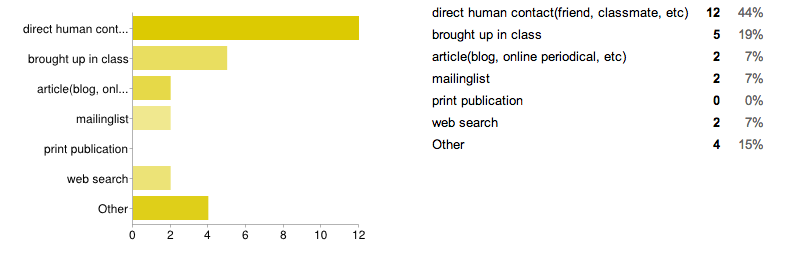
\includegraphics[width=120mm]{chapters/img/importance_of_personal_touch.png}
\caption{Importance of personal touch}
\label{fig:personal_touch}
\end{figure}

Personal contact was also an important outreach method for 46\% of the projects surveyed, and we further examined whether this finding was related to the size of the group. An open-ended survey question about project outreach was qualitatively coded for personal contact, with responses indicating effort such as small in-person meetings and/or project member attendance and outreach at hackathons, workshops, conferences, and other community events that were not only held online. We did not find a dependence between group size and outreach through personal contact (Fisher's Exact Test, $p = 0.55$). This suggests that both large and small groups rely on various types of in-person outreach to recruit new contributors. Since these organized group meetings are a common first contact point for many potential contributors, further research is needed to identify how different types and approaches to personal modes of outreach impact the recruitment of individuals with specific skills or motivations.

Most respondents have had a physical contact with at least one of the projects contributors. This can have been in the university environment such as a Talk and by chatting with classmates or at work. This was the initial trigger that made them know about the project and at the same time breaking down entry barriers since it was easier to get information when needed. Therefore many projects joined by students are somehow connected to the Bay Area.